%
% File acl2020.tex
%
%% Based on the style files for ACL 2020, which were
%% Based on the style files for ACL 2018, NAACL 2018/19, which were
%% Based on the style files for ACL-2015, with some improvements
%%  taken from the NAACL-2016 style
%% Based on the style files for ACL-2014, which were, in turn,
%% based on ACL-2013, ACL-2012, ACL-2011, ACL-2010, ACL-IJCNLP-2009,
%% EACL-2009, IJCNLP-2008...
%% Based on the style files for EACL 2006 by 
%%e.agirre@ehu.es or Sergi.Balari@uab.es
%% and that of ACL 08 by Joakim Nivre and Noah Smith

\documentclass[11pt,a4paper]{article}
\usepackage[hyperref]{acl2020}
\usepackage{times}
\usepackage{latexsym}
\renewcommand{\UrlFont}{\ttfamily\small}

\usepackage{float} % for floating
\usepackage{graphicx}% so it makes black blobs
\graphicspath{ {images/} }
\usepackage{caption}
\usepackage{subcaption}
\usepackage{amsmath}


% This is not strictly necessary, and may be commented out,
% but it will improve the layout of the manuscript,
% and will typically save some space.
\usepackage{microtype}

\aclfinalcopy % Uncomment this line for the final submission
%\def\aclpaperid{***} %  Enter the acl Paper ID here

%\setlength\titlebox{5cm}
% You can expand the titlebox if you need extra space
% to show all the authors. Please do not make the titlebox
% smaller than 5cm (the original size); we will check this
% in the camera-ready version and ask you to change it back.

\newcommand\BibTeX{B\textsc{ib}\TeX}

\title{Predicting Diabetes using Adaptive-Network-based Fuzzy Inference System (ANFIS)}

\author{Krishna Chaitanya Reddy Tamataam \\
  Department of Mathematics \\
  IIT Delhi \\
  Delhi 110016, India \\
  \texttt{mt6180785@maths.iitd.ac.in} \\\And
  Subhalingam D \\
  Department of Mathematics \\
  IIT Delhi \\
  Delhi 110016, India \\
  \texttt{mt1180770@maths.iitd.ac.in} \\}

\date{}

\begin{document}

\newcommand{\varacctrain}{$85.42\%$}
\newcommand{\varacctest}{$81.30\%$}
\newcommand{\varftrain}{$78.44\%$}
\newcommand{\varftest}{$74.72\%$}
\newcommand{\varprectrain}{$81.04\%$}
\newcommand{\varprectest}{$70.83\%$}
\newcommand{\varrectrain}{$76.00\%$}
\newcommand{\varrectest}{$79.06\%$}
\newcommand{\varlosstrain}{$0.33549$}
\newcommand{\varlosstest}{$0.43418$}

\newcommand{\vargithubrepo}{\url{https://github.com/subhalingamd/ANFIS}}

\maketitle
\begin{abstract}
We studied the Adaptive-Network-based Fuzzy Inference System (ANFIS) proposed by \newcite{anfis}. We implemented a simple version of ANFIS for Diabetes predictor with Gaussian membership functions and tuned it. Our model had a test accuracy of \varacctest, train accuracy of \varacctrain, test F1-score of \varftest { }and train F1-score of \varftrain. We further analysed the variation of performance metrics and losses with epochs, constructed the confusion matrix, plotted graphs of the membership functions learnt by the model and discussed our observations.
\end{abstract}



\section{Introduction}
In the recent times, due to availability of large amount of data and high computational power, Artificial Intelligence (AI) and Machine Learning (ML) algorithms play a very important role in automation. From basic neural networks to predict a simple non-linear functions to speech recognition using Recurrent Neural Network (RNN), there are several applications of AI that we use in our day-to-day lives. In today's world these models have been trained rigorously and have achieved high accuracy. But a feature used for classification cannot be a crisp value exactly, i.e., there is some amount of \textit{fuzziness} involved \cite{fuzzy:zadeh}. To account for this, we use membership function to estimate the relatedness of an element to a set. This feature plays a very important role in identifying unclear examples in the dataset. Fuzzy neural networks (FNN) combine the Fuzzy Logic and Neural networks in single model. We study Adaptive-Network-based Fuzzy Inference System (ANFIS) \cite{anfis} and implement a model to that predicts whether a person is having diabetes or not. ANFIS has many applications in field of geo-engineering studies, such as soil analysis (predicting friction angles of soil), variations in salinity of sea with temperature, pressure and other factors. In the field of image detection, it is used for identifying Breast cancer.
% Even MATLAB has a tool box for ANFIS framework.


\section{Model}
\subsection{Architecture}
Adaptive-Network-based Fuzzy Inference System (ANFIS) is derived from the first order Takagi-Sugeon fuzzy inference system \cite{Sugeno}. The main advantage of such a system over other inference system is that the parameters used for its membership functions can be changed (different membership functions, described in Section \ref{sec:mf}, can be used for each fuzzy rule). Hence we can apply Machine Learning (ML) algorithms to train these parameters and build a model that fits into the given dataset. Moreover, ANFIS can be stacked with any other Deep Learning models, which makes it more interesting to study and unique from other Fuzzy Neural Networks.
% \subsection{Layers}

\begin{figure}[htbp]
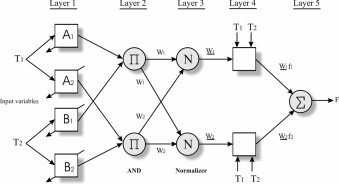
\includegraphics[width=\columnwidth]{arch1.jpg}
\caption{\label{fig:arch1} Architecture of ANFIS}
\end{figure}

ANFIS is made up of \textit{five} layers as discussed in the following subsections.
\subsubsection{Input layer}
This contains the input features of the data used by the model. The data has to be standardised before it is being fed to the model. Mathematically, our input data will be a $n$ dimensional vector for each example (data point).

% For this model, we have used 6 features from the 8 namely number of times pregnant,Plasma Glucose Concentration,Triceps Skin fold thickness,two hour serum insulin,BMI(body mass index),Diabetes Pedigree  and age.From of correlation matrix of these features we exclude No of times pregnant and age from the consideration.

\subsubsection{Fuzzification Layer}
\label{sec:fuzzlayer}
This layer is made up of $mn$ nodes (where $m$ is the desired number of fuzzy rules and $n$ is the number of input features). For every input feature $i$, ($i = 1,2, \dots ,n$) there are nodes $a_{ij}$ where $j = 1,2, \dots ,m$. A Gaussian membership function ([ \ref{formula:gmf}] in Section \ref{sec:mf}), with trainable parameters $\mu$ (mean)  and $\sigma^2$ (variance), is applied to the input features to obtain the output for this layer.

\subsubsection{Rule Layer}.
This layer takes the product (algebraic intersection, $\cap_a$) of the respective rules obtained in the previous layer. The output of this layer is fed as input for the next layer.

Each node {$a_j$} in this layer, it2 takes {$x_{1j},x_{2j}...... x_{nj}$} from the previous layer,
where $n$ is the number of features and $j = 1,2, \dots, m$, where $m$ is the number of fuzzy rules. It gives product of all these values, i.e., $a_j = \prod_{i=1}^n x_{ij}$, as the output which is then normalised.

\subsubsection{De-fuzzification layer}
It has $m$ nodes which is the number of fuzzy rules. As the name says, this layer is used for defuzzification. Each node takes the corresponding previous node output and the input layer values and does the following $(a_0+a_1x_1+a_2.x_2+ \dots + a_nx_n)$.$w$ where $w$ is the weight of the corresponding rule layer and  $a_0,a_1 , a_2 , \dots,  a_{n}$ are trainable parameters.

\subsubsection{Output layer}
All the outputs from previous layer is added and an activation function (sigmoid function, in our case) is applied.

\subsection{Equations for Forward pass}
\subsubsection{Layer 1}
% For each node $i$,
For $n$ input features $x_i$  ($i = 1,2, \dots ,n$),
\begin{align}
    \text{Input: } & x_1,x_2,\dots,x_n \\
    \text{Output: } & x_1,x_2,\dots,x_n
\end{align}

\subsubsection{Layer 2}
For each node $a_{ij}$ where $i = 1,2, \dots ,n$ and $j = 1,2, \dots ,m$
\begin{align}
    \text{Input: } & x_i \\
    \text{Output: } & N_{i1}(x_i),N_{i2}(x_i),......N_{im}(x_i)
\end{align}
where $N_{ij}$ is the Gaussian membership function ([ \ref{formula:gmf}] in Section \ref{sec:mf}) with mean $\mu_{ij}$ and variance $\sigma_{ij}^2$.

\subsubsection{Layer 3}
For each node $j$ ($j = 1,2, \dots ,m$),
\begin{align}
    \text{Input: } & w_{1j}, w_{2j}, \dots, w_{nj} \\
    ~ & w_{j} = w_{1j} \cdot w_{2j} \cdots w_{nj} \\
    ~ & sum =  w_{1}+w_{2}+ \dots + w_{m} \\
    \text{Output: } & w^*_j = w_{j}/sum
\end{align}
Here, $w^*_j$ is the normalized weight.

\subsubsection{Layer 4}
for each $j$ ($j = 1,2, \dots ,m$),
\begin{align}
    \text{Input: } & f_j= a_{0j}+a_{1j}x_1+\dots+a_{nj}x_{n} \\
    \text{Output: } & w^*_j\dot f_j
\end{align}
where $a_0,a_1,\dots,a_n$ are trainable parameters.

\subsubsection{Layer 5}
for each $j$ ($j = 1,2, \dots ,m$)
\begin{align}
    \text{Input: } & X = \sum_{j=1}^{m} w^*_j\dot f_j \\
    \text{Output: } & \sigma({X})
\end{align}
where $\sigma (x) = \frac{1}{1+e^{-x}}$ is the sigmoid function. If $x>0$, $\sigma(x)>0.5$, so we assign a label $1$ to such an input (and $0$ otherwise).


\subsection{Membership functions}
\label{sec:mf}
Gaussian membership function is the widely used membership function. Yet, other membership functions like Generalized Bell membership function, Triangular fuzzy number, Trapezoidal fuzzy number, etc., can also be applied. However, it is recommended to choose a function with smooth curves, so that they are differentiable (helpful for optimizer while training), and it also helps us to learn non-linear functions. In Figure \ref{fig:gmf1}, \ref{fig:gmf1}a represents Gaussian membership function, \ref{fig:gmf1}b represents a combination of two Gaussian functions and \ref{fig:gmf1}c represents Generalised bell function.

Given below is Gaussian Membership Function we used in the Fuzzification Layer (Section \ref{sec:fuzzlayer})\\

\begin{align}\label{formula:gmf}
    N(x) = \frac{1}{{\sigma \sqrt {2\pi } }}e^{{{ - \left( {x - \mu } \right)^2 } \mathord{\left/ {\vphantom {{ - \left( {x - \mu } \right)^2 } {2\sigma ^2 }}} \right. \kern-\nulldelimiterspace} {2\sigma ^2 }}}
\end{align}
where $\mu$ is the mean and $\sigma ^2$ is the variance.


\begin{figure*}[htbp]
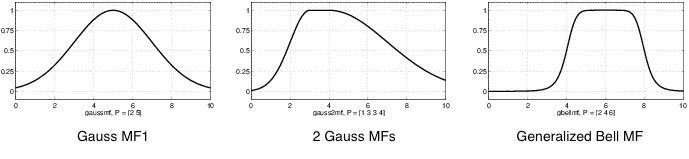
\includegraphics[width=2\columnwidth]{gbellandgaussmfs.png}
\caption{\label{fig:gmf1} Different Membership Functions that can be used}
\end{figure*}

\section{Experiment}
\subsection{Dataset}
We use the "\textit{Pima Indians Diabetes Database}" from Kaggle \footnote{\url{https://www.kaggle.com/uciml/pima-indians-diabetes-database}}. The dataset contains $768$ examples and $8$ features (\textit{plus one} outcome) as mentioned in Table \ref{tab:dataset-desc}. {\em It is worthy to note that this dataset only consists of females who are at least 21 years old}.

\begin{table}[h]
\centering
\begin{tabular}{| p{2cm} | p{4.7cm}|}
\hline \textbf{Feature} & \textbf{Short Description} \\ \hline
{\em Pregnancies} & Number of times pregnant \\ \hline
{\em Glucose} & Plasma glucose concentration a 2 hours in an oral glucose tolerance test \\ \hline
{\em Blood Pressure} & Diastolic blood pressure (mm Hg) \\ \hline
{\em Skin Thickness} & Triceps skin fold thickness (mm) \\ \hline
{\em Insulin} & 2-hour serum insulin ($mu$ U/ml) \\ \hline
{\em BMI}& Body mass index (weight in kg/(height in m)$^2$) \\ \hline
{\em Diabetes Pedigree Function} & Diabetes pedigree function \\ \hline
{\em Age} & Age (years) \\ \hline
{\em Outcome} & Class variable (0 or 1) \\ 
\hline
\end{tabular}
\caption{\label{tab:dataset-desc} Description of features in Dataset}
\end{table}

\subsection{Pre-processing}
\label{sec:process}
We split the dataset into train and test data using \texttt{ sklearn.model\_selection.train\_test \_split()} The model requires each feature to have a mean $0$ and standard deviation $1$. Hence, we standardize each column of the dataset before using it.

It was observed that the dataset did not have any missing data-so no additional processing were necessary.



\subsection{Settings}

% some placeholders
\newcommand{\varsplit}{$0.16$}
\newcommand{\varseed}{$2021$}
\newcommand{\varfuzzyrules}{$14$}
\newcommand{\varlossfn}{Binary Cross Entropy }
\newcommand{\varoptimizer}{Adam Optimizer }
\newcommand{\varalpha}{$0.01$ }
\newcommand{\varepochs}{$1000$ }
\newcommand{\varepochinterval}{$10$ }
\newcommand{\varmf}{Gaussian }

We conducted our experiment with the following hyperparameters:
\begin{itemize}
    \item The model was implemented\footnote{Code available at \vargithubrepo} in Python using TensorFlow (v1.15.4) \cite{tensorflow}. Scikit-learn (v0.24.0) \cite{scikit-learn} was used to compute the metric values and Matplotlib (v3.0.3) \cite{matplotlib} was used to plot graphs.
    \item As mentioned in Section \ref{sec:process}, we used \texttt{ sklearn.model\_selection.train\_ test\_split()} with \texttt{test\_split} set to \varsplit. Moreover, \texttt{random\_state} was set to \varseed.
    \item Total number of fuzzy rules used in the model was set to \varfuzzyrules.
    \item \varlossfn was the loss function used.
    \item \varoptimizer was used with learning parameter $\alpha =$ \varalpha to optimize the loss function in \varepochs epochs.
    \item Data points for plotting graphs in Section \ref{sec:results} were taken at every \varepochinterval epochs.
    \item \varmf membership function was used for each fuzzy rule. The weights, $\mu$, $\sigma$ were randomly initialised from normal distribution.
    
\end{itemize}

Additionally, we omit or discard the \textit{Pregnancies} column from the dataset, while building our model, as we thought it doesn't have a direct relation with the disease of interest.

After splitting the dataset, we analysed the number of data points belonging to each class in train and test set and mentioned it in Table \ref{tab:dataset-distr}.

\begin{table}[h]
\centering
\begin{tabular}{| l | c c |}
\hline ~ & \textbf{\#1 (Positive)} & \textbf{\#0 (Negative)} \\ \hline
Train & $225$ & $420$ \\
Test & $43$ & $80$ \\ \hline
\textbf{Total} & $268$ & $500$ \\
\hline
\end{tabular}
\caption{\label{tab:dataset-distr} Distribution of data in train and test set}
\end{table}

% Train:  { 0: 420, 1: 225 }
% Test:   { 0: 80,  1: 43  }

\subsection{Results}
\label{sec:results}
We use the following notations to define the performance metrics we use in this report:
\begin{itemize}
    \item \textbf{TP} (True Positive): Model predicts Positive and it is actually Positive.
    \item \textbf{FP} (False Positive): Model predicts Positive but it is actually Negative.
    \item \textbf{FN} (False Negative): Model predicts Negative but it is actually Positive.
    \item \textbf{TN} (True Negative): Model predicts Negative and it is actually Negative.
\end{itemize}

Now, we define the performance metrics of our interest.
\begin{table}[htpb]
\centering
\begin{tabular}{lcl}
Accuracy & = & $\frac{TP + TN}{TP + FP + FN + TN}$ \\
~ & ~ & ~ \\
Precision & = & $\frac{TP}{TP + FP}$ \\
~ & ~ & ~ \\
Recall & = & $\frac{TP}{TP + FN}$ \\
~ & ~ & ~ \\
F1-Score & = & $\frac{2 \times \text{Precision} \times
\text{Recall}}{\text{Precision}+\text{Recall}}$ \\
\end{tabular}
\end{table}

The performance and losses of model on train and test set is given in Table \ref{tab:performance}.

\begin{table}[h]
\centering
\begin{tabular}{| l | c | c |}
\hline ~ & \textbf{Test} & \textbf{Train} \\ \hline
Accuracy & \varacctest & \varacctrain \\
Precision & \varprectest & \varprectrain \\
Recall & \varrectest & \varrectrain \\
F1-score & \varftest & \varftrain \\ \hline
Loss & \varlosstest & \varlosstrain \\ \hline
\end{tabular}
\caption{\label{tab:performance} Performance and Losses of the model}
\end{table}

We have constructed the confusion matrix in Figure \ref{fig:cf} (for test set in Figure \ref{fig:cf:test} and train set in Figure \ref{fig:cf:train}). We plotted the losses in Figure \ref{fig:loss-graph} and performance metrics (accuracy, F1-score, precision, recall) in Figure \ref{fig:perform-graph} over number of epochs, for both test and train sets. The graph of membership functions learnt by each fuzzy rule for the given features are plotted in Figure \ref{fig:rules}.

\begin{figure}[htbp]
\begin{subfigure}{\columnwidth}
  \centering
  % include first image
  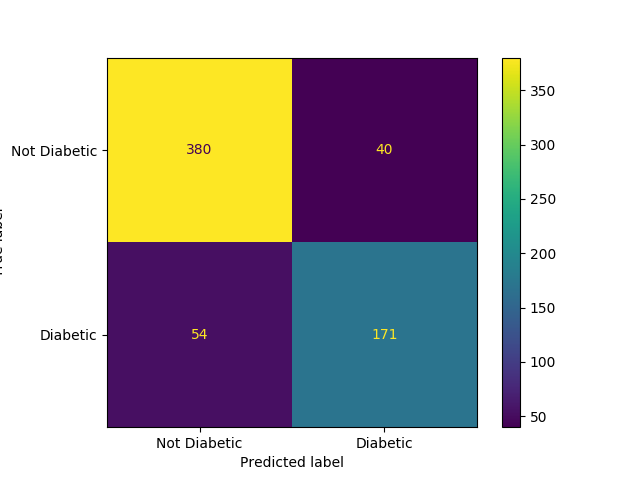
\includegraphics[width=\columnwidth,keepaspectratio]{cf_train-epoch1000.png}  
  \caption{Train set}
  \label{fig:cf:test}
\end{subfigure}
\begin{subfigure}{\columnwidth}
  \centering
  % include second image
  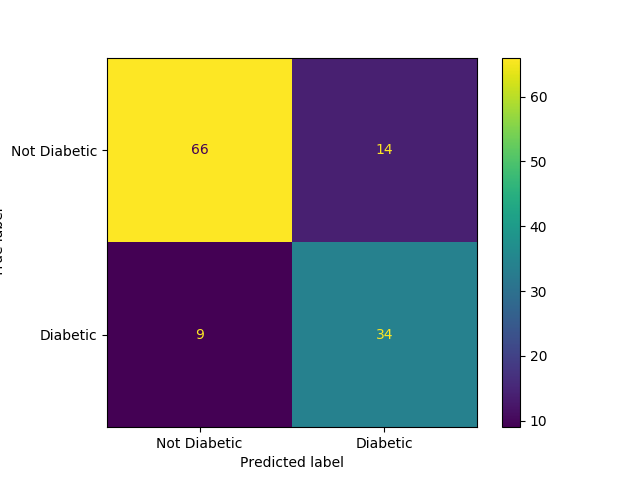
\includegraphics[width=\columnwidth,keepaspectratio]{cf_test-epoch1000.png}
  \caption{Test set}
  \label{fig:cf:train}
\end{subfigure}
\caption{Confusion Matrix}
\label{fig:cf}
\end{figure}

\begin{figure}[hbtp]
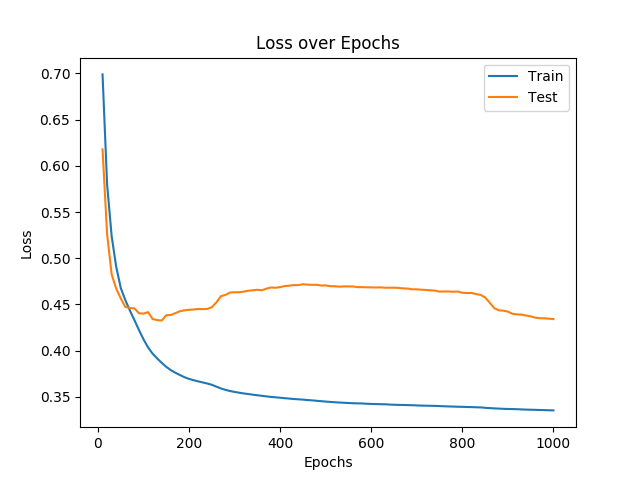
\includegraphics[width=\columnwidth]{loss.png}
\caption{\label{fig:loss-graph} Loss over epochs}
\end{figure}

\begin{figure*}[htbp]
\begin{subfigure}{\columnwidth}
  \centering
  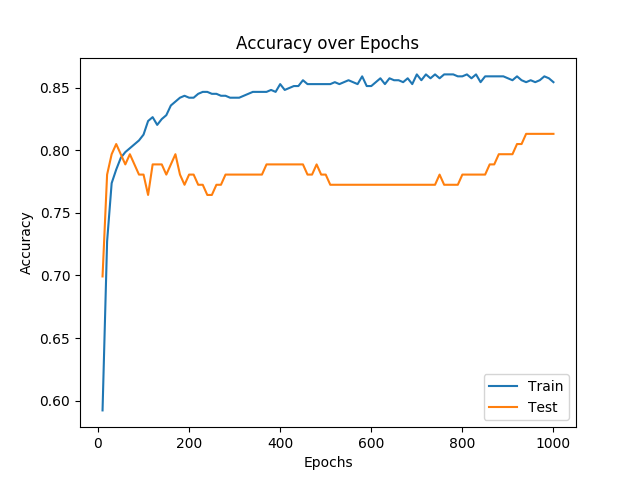
\includegraphics[width=\columnwidth,keepaspectratio]{acc.png}  
  \caption{Accuracy}
  \label{fig:perform-graph:acc}
\end{subfigure}
\begin{subfigure}{\columnwidth}
  \centering
  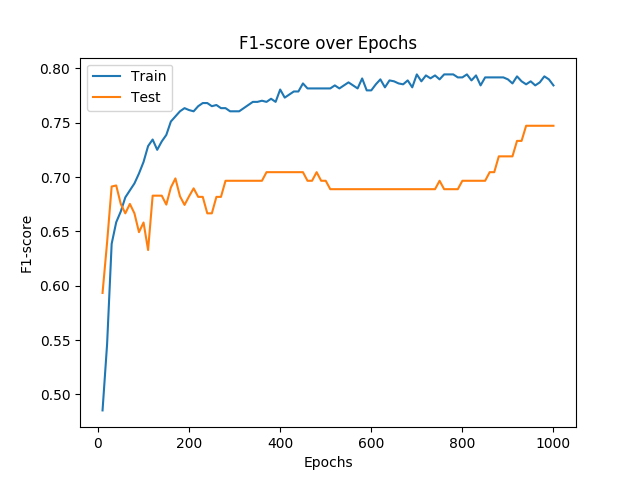
\includegraphics[width=\columnwidth,keepaspectratio]{f1.png}
  \caption{F1-score}
  \label{fig:perform-graph:f1}
\end{subfigure}
\begin{subfigure}{\columnwidth}
  \centering
  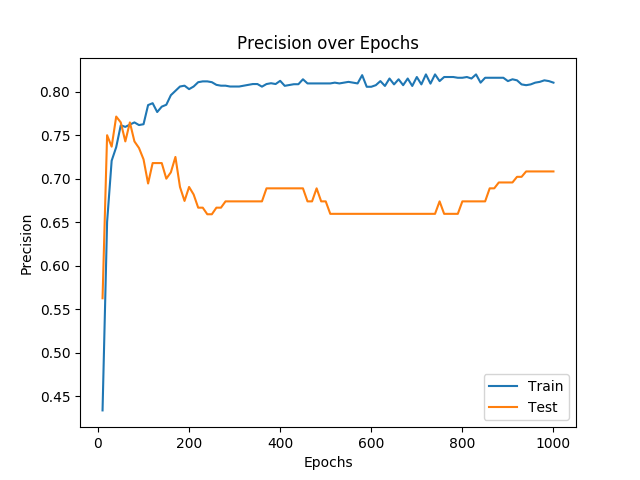
\includegraphics[width=\columnwidth,keepaspectratio]{precision.png}
  \caption{Precision}
  \label{fig:perform-graph:prec}
\end{subfigure}
\begin{subfigure}{\columnwidth}
  \centering
  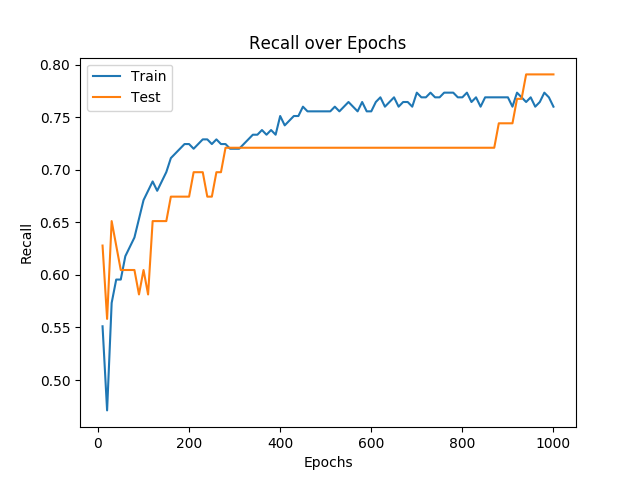
\includegraphics[width=\columnwidth,keepaspectratio]{recall.png}
  \caption{Recall}
  \label{fig:perform-graph:rec}
\end{subfigure}
\caption{Performance metrics over epochs}
\label{fig:perform-graph}
\end{figure*}


\begin{figure*}[htbp]
\begin{subfigure}{\columnwidth}
  \centering
  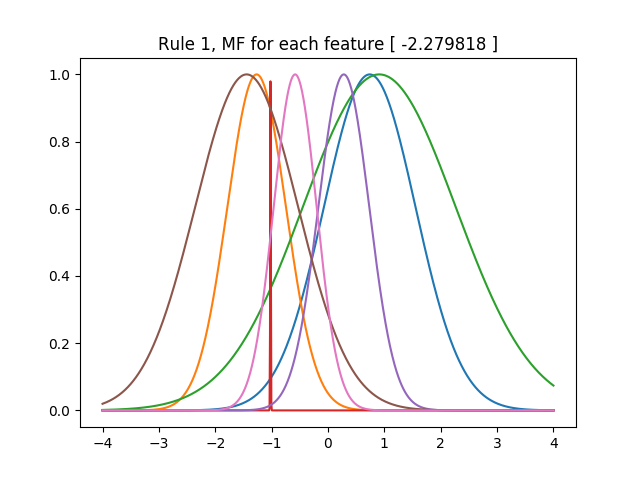
\includegraphics[width=\columnwidth,keepaspectratio]{rule-1.png}  
  \caption{Rule 1}
  \label{fig:rules:rule-1}
\end{subfigure}
\begin{subfigure}{\columnwidth}
  \centering
  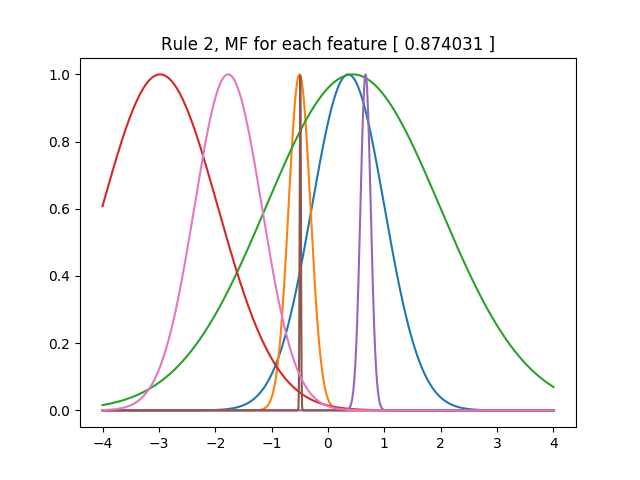
\includegraphics[width=\columnwidth,keepaspectratio]{rule-2.png}  
  \caption{Rule 2}
  \label{fig:rules:rule-2}
\end{subfigure}
\begin{subfigure}{\columnwidth}
  \centering
  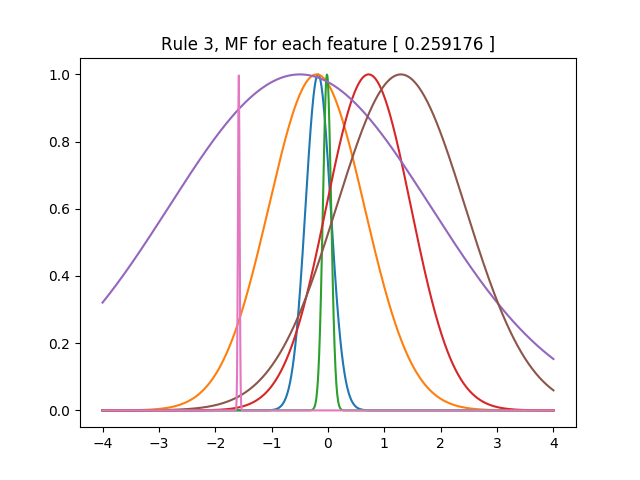
\includegraphics[width=\columnwidth,keepaspectratio]{rule-3.png}  
  \caption{Rule 3}
  \label{fig:rules:rule-3}
\end{subfigure}
\begin{subfigure}{\columnwidth}
  \centering
  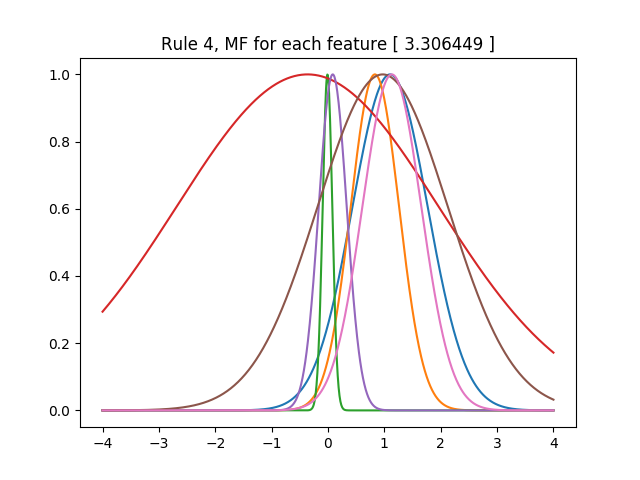
\includegraphics[width=\columnwidth,keepaspectratio]{rule-4.png}
  \caption{Rule 4}
  \label{fig:rules:rule-4}
\end{subfigure}
\begin{subfigure}{\columnwidth}
  \centering
  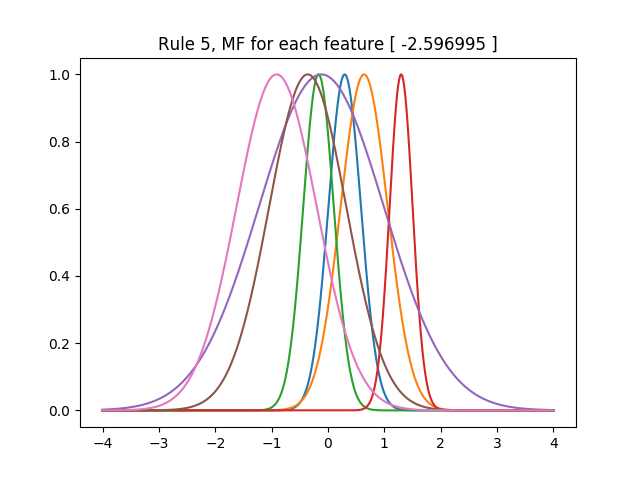
\includegraphics[width=\columnwidth,keepaspectratio]{rule-5.png}  
  \caption{Rule 5}
  \label{fig:rules:rule-5}
\end{subfigure}
\begin{subfigure}{\columnwidth}
  \centering
  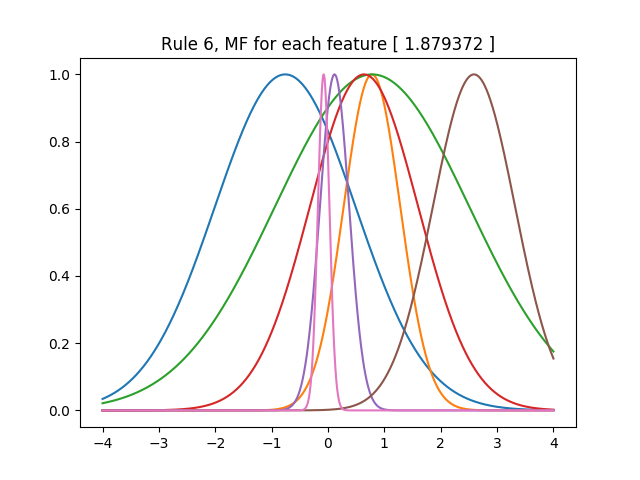
\includegraphics[width=\columnwidth,keepaspectratio]{rule-6.png}
  \caption{Rule 6}
  \label{fig:rules:rule-6}
\end{subfigure}
\end{figure*}


\begin{figure*}[htbp]
\ContinuedFloat
\begin{subfigure}{\columnwidth}
  \centering
  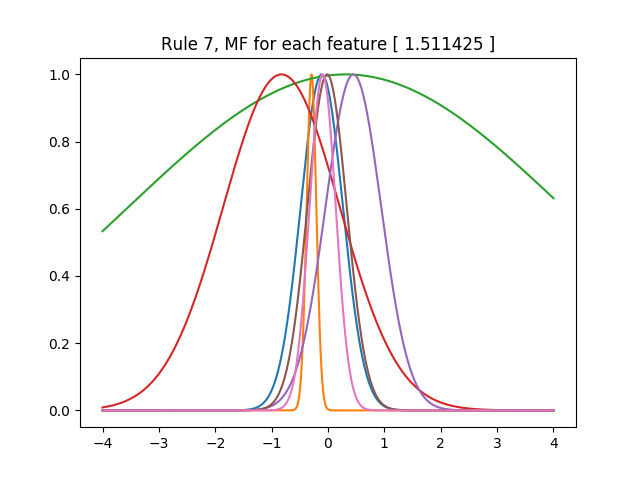
\includegraphics[width=\columnwidth,keepaspectratio]{rule-7.png}  
  \caption{Rule 7}
  \label{fig:rules:rule-7}
\end{subfigure}
\begin{subfigure}{\columnwidth}
  \centering
  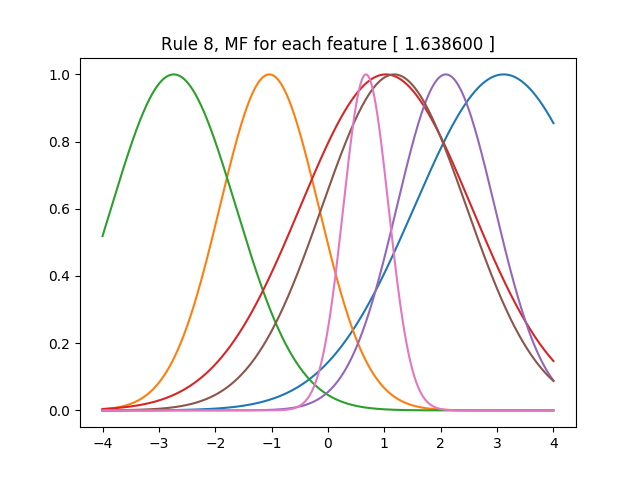
\includegraphics[width=\columnwidth,keepaspectratio]{rule-8.png}  
  \caption{Rule 8}
  \label{fig:rules:rule-8}
\end{subfigure}
\begin{subfigure}{\columnwidth}
  \centering
  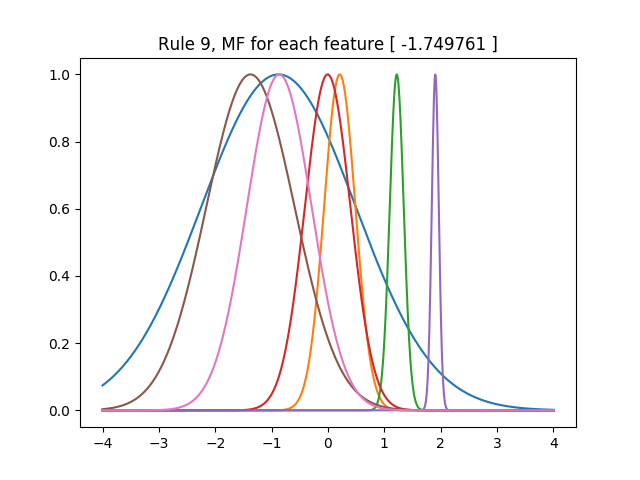
\includegraphics[width=\columnwidth,keepaspectratio]{rule-9.png}  
  \caption{Rule 9}
  \label{fig:rules:rule-9}
\end{subfigure}
\begin{subfigure}{\columnwidth}
  \centering
  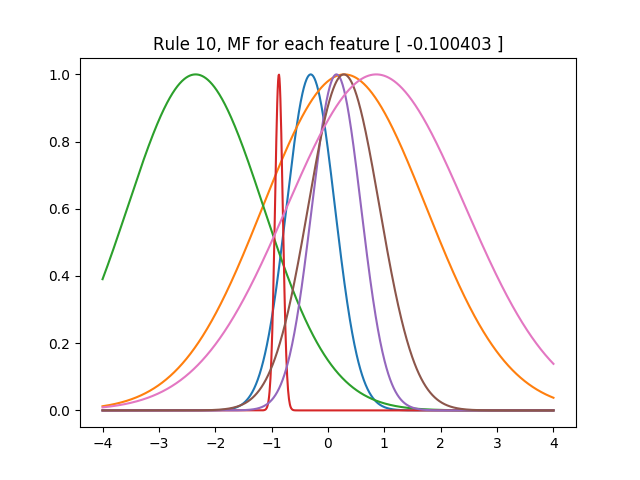
\includegraphics[width=\columnwidth,keepaspectratio]{rule-10.png}
  \caption{Rule 10}
  \label{fig:rules:rule-10}
\end{subfigure}
\begin{subfigure}{\columnwidth}
  \centering
  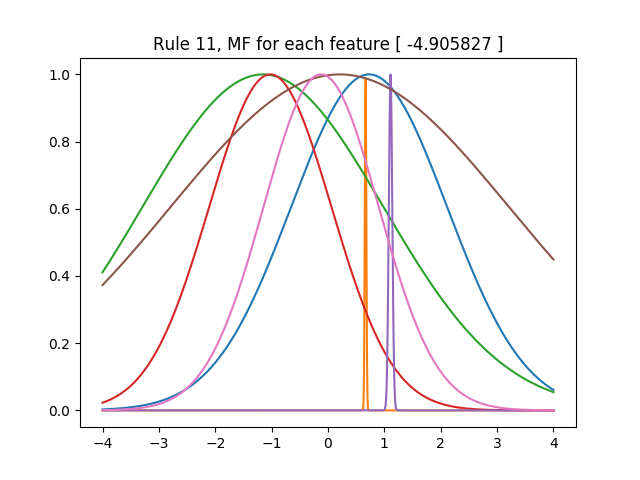
\includegraphics[width=\columnwidth,keepaspectratio]{rule-11.png}  
  \caption{Rule 11}
  \label{fig:rules:rule-11}
\end{subfigure}
\begin{subfigure}{\columnwidth}
  \centering
  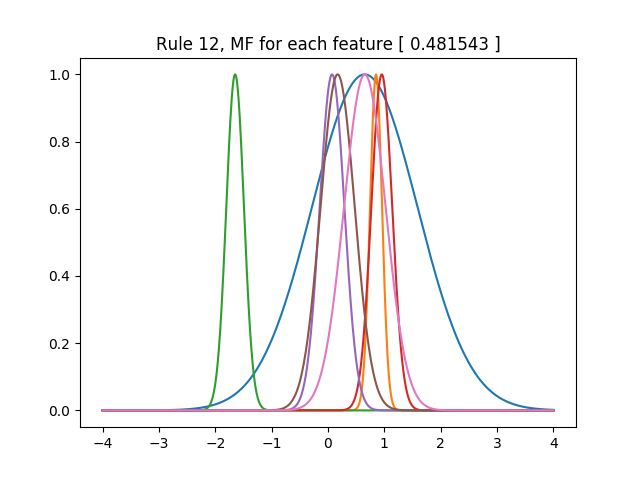
\includegraphics[width=\columnwidth,keepaspectratio]{rule-12.png}
  \caption{Rule 12}
  \label{fig:rules:rule-12}
\end{subfigure}
% \caption{Membership Functions of Fuzzy Rules learnt}
% \label{fig:rules}
\end{figure*}

\begin{figure*}[htbp]
\ContinuedFloat
\begin{subfigure}{\columnwidth}
  \centering
  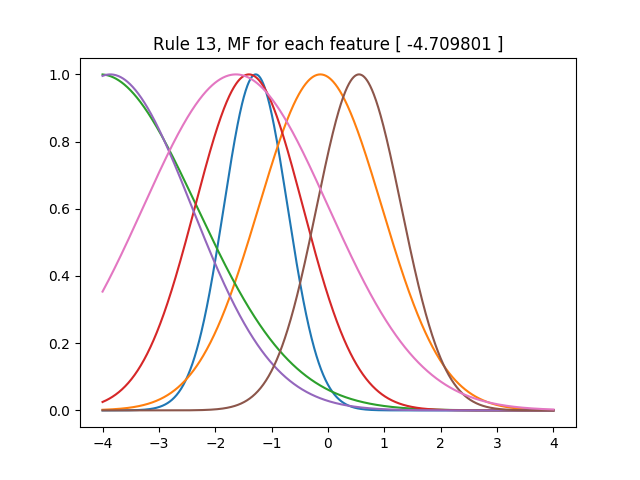
\includegraphics[width=\columnwidth,keepaspectratio]{rule-13.png}  
  \caption{Rule 13}
  \label{fig:rules:rule-13}
\end{subfigure}
\begin{subfigure}{\columnwidth}
  \centering
  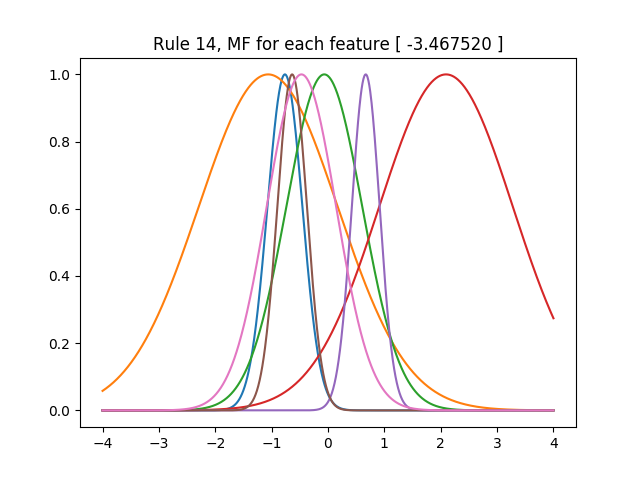
\includegraphics[width=\columnwidth,keepaspectratio]{rule-14.png}
  \caption{Rule 14}
  \label{fig:rules:rule-14}
\end{subfigure}
\caption{Membership Functions of Fuzzy Rules learnt}
\label{fig:rules}
\end{figure*}







Additionally, the following were observed:
\begin{itemize}
    \item The model's performance was found to be too sensitive to the initialisation of the parameters. Since we initialised them randomly, we observed that there was a lot of fluctuation in terms of accuracy and F1-score when we ran them multiple times.
    \item Just like any Machine Learning models, we observed that lower number of fuzzy rules led to underfitting while increasing them too much led to overfitting. This can be reasoned similar to the underfitting (or overfitting) case when we choose too less (or too many) hidden units in a Neural Network.
    % \item The accuracy first increases, reaches a minimum and then starts decreasing on the train set. It is required to stop the training when the maxima is reached (early stopping). This is an example of bias-variance tradeoff.
\end{itemize}




\section{Possible Additions}
We can build a similar image classifier for breast cancer detection. However, for images, the number of input features (total number of pixels) in image will be too high. One approach would be to reduce the these dimensions and use the reduced features as the input to our model. This can be achieved with some Dimension Reduction techniques like Principal Component Analysis (PCA) \cite{PCA:12}. 
% This technique involves finding the eigen-value of eigen-vectors for the co-varaince matrix.


\section{Conclusion}
We studied the working of ANFIS and applied the concepts to a real-life dataset and reported our results in Section \ref{sec:results}, after training over 100 different models. In medical domain, we expect the recall to be high, as we do not want to miss a positive case, even at the cost of false positive.

\cleardoublepage

\section*{Acknowledgments}
This project was inspired from a paper title "{\em Application of Adaptive Neuro-Fuzzy Inference System for diabetes classification and prediction}" by Oana Geman, Iuliana Chiuchisan, and Roxana Toderean. However, the work done in this report is ours (unless cited) and the paper mentioned above helped us to understand some applications of ANFIS and choose a dataset.

\bibliographystyle{acl_natbib}
\bibliography{ref}

\end{document}
